\section{Darbo pasiskirstymo semestro metu analizė}

Su \ref{lst:months} programa susumavus, kiek laiko buvo skirta kiekvienam
iš dalykų kiekvieną mėnesį, gauti rezultatai pateikti
\ref{tab:months} lentelėje ir \ref{fig:semester_work} paveikslėliuose.

\begin{sidewaystable}[ht!]
  \centering
  \begin{tabular}{|l|c|c|c|c|c|c|}
\hline
&1&2&3&4&5&6\\
Dalyko pavadinimas&sausis&vasaris&kovas&balandis&gegužė&birželis\\
\hline
Algoritmavimo seminaras&5:20:00&&&&3:13:00&2:52:00\\
Psichologijos įvadas&&8:00:00&8:00:00&12:21:00&18:54:00&17:11:00\\
Programų sistemų inžinerija&&12:53:00&51:03:00&17:50:00&53:46:00&31:27:00\\
Interneto technologijos&&9:28:00&23:14:00&20:32:00&21:09:00&17:20:00\\
Tikimybių teorija ir matematinė statistika&&11:05:00&18:36:00&24:39:00&16:58:00&33:43:00\\
Operacinės sistemos&&23:21:00&53:51:00&40:32:00&95:51:00&\\
Matematinė logika&&8:10:00&14:00:00&11:10:00&14:00:00&7:09:00\\
Vokiečių kalba&&10:26:00&47:13:00&23:35:00&37:21:00&7:09:00\\
\hline
  \end{tabular}
  \caption{Dalykams skirtas laikas.}
  \label{tab:months}
\end{sidewaystable}

\begin{figure}[H]
  \centering

  \subfloat[Algoritmavimo seminaras]{%
    \label{fig:semester_work:algoritmavimo_seminaras}%
    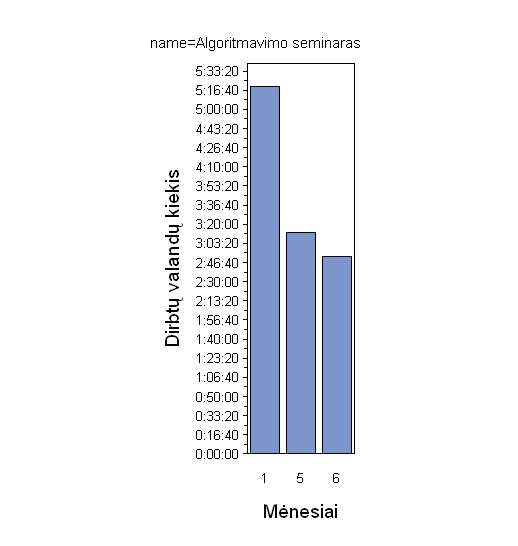
\includegraphics[width=0.3\linewidth]{%
    images/months/Algoritmavimo_seminaras.png}}
  \subfloat[Interneto technologijos]{%
    \label{fig:semester_work:interneto_technologijos}%
    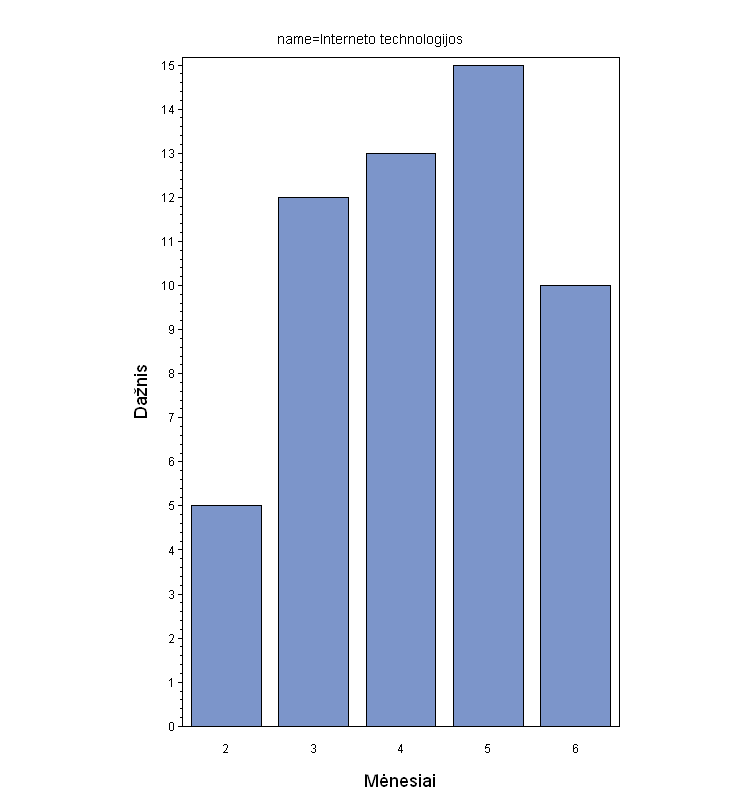
\includegraphics[width=0.3\linewidth]{%
    images/months/Interneto_technologijos.png}}
  \subfloat[Matematinė logika]{%
    \label{fig:semester_work:matematine_logika}%
    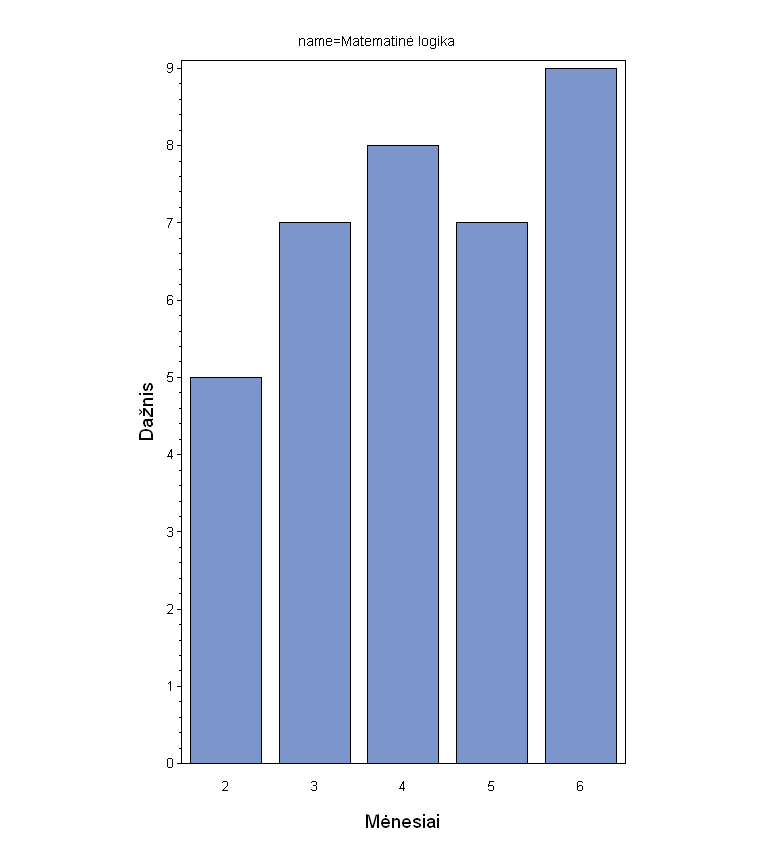
\includegraphics[width=0.3\textwidth]{%
      images/months/Matematine_logika.png}}

  \subfloat[Operacinės sistemos]{%
    \label{fig:semester_work:operacines_sistemos}%
    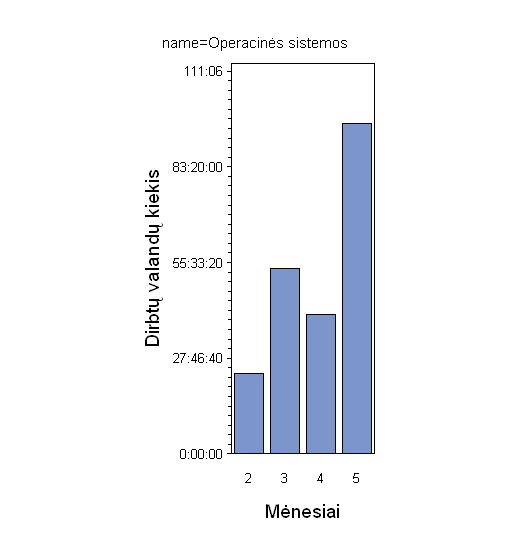
\includegraphics[width=0.3\linewidth]{%
    images/months/Operacines_sistemos.png}}
  \subfloat[Programų sistemų inžinerija]{%
    \label{fig:semester_work:programu_sistemu_inzinerija}%
    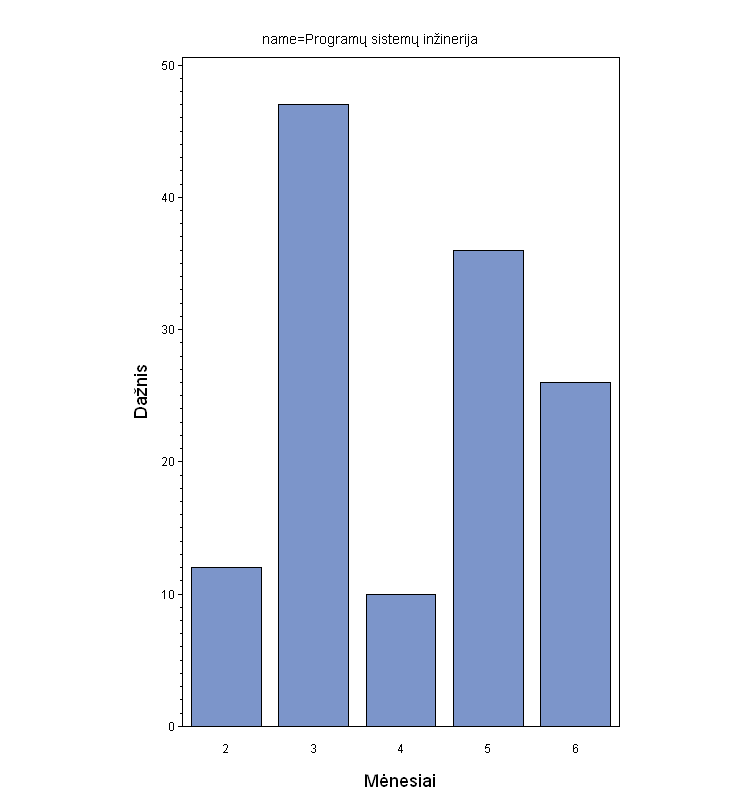
\includegraphics[width=0.3\linewidth]{%
    images/months/Programu_sistemu_inzinerija.png}}
  \subfloat[Psichologijos įvadas]{%
    \label{fig:semester_work:psichologijos_ivadas}%
    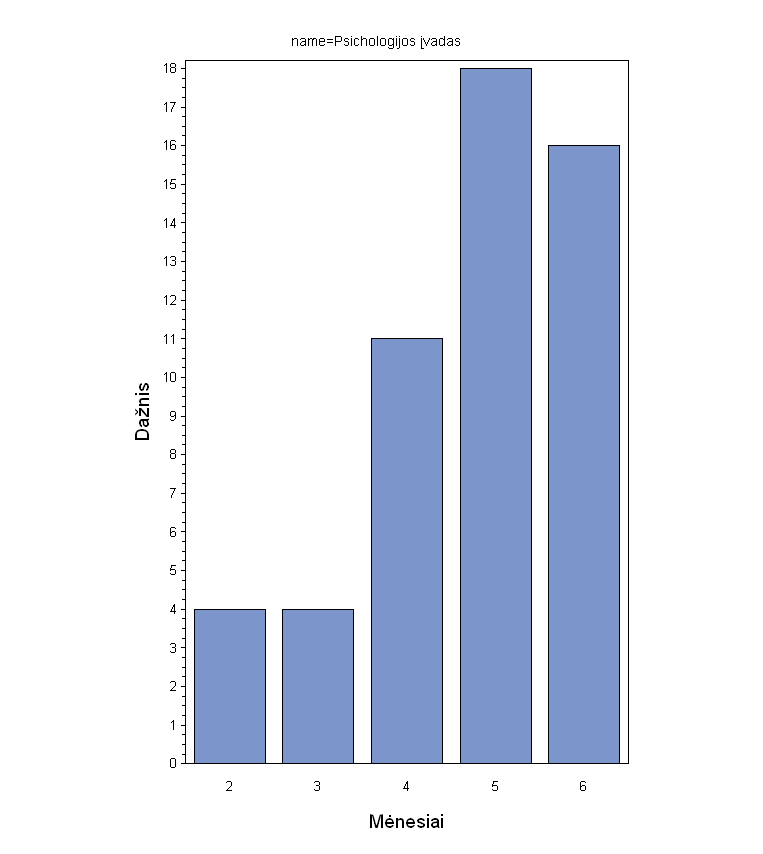
\includegraphics[width=0.3\textwidth]{%
      images/months/Psichologijos_ivadas.png}}

  \subfloat[Tikimybių teorija ir matematinė statistika]{%
    \label{fig:semester_work:tikimybiu_teorija}%
    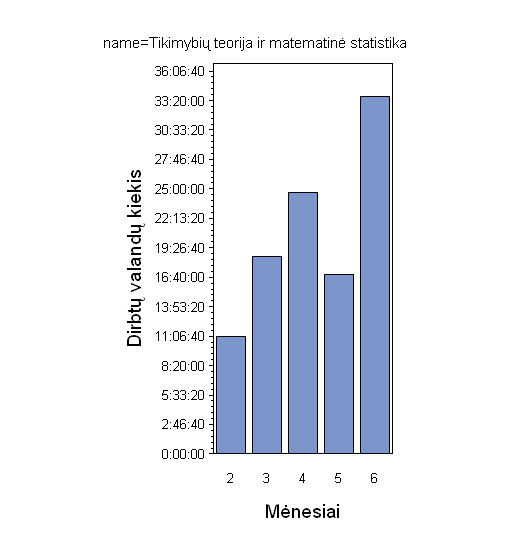
\includegraphics[width=0.3\linewidth]{%
    images/months/Tikimybiu_teorija_ir_matematine_statistika.png}}
  \subfloat[Vokiečių kalba]{%
    \label{fig:semester_work:vokieciu_kalba}%
    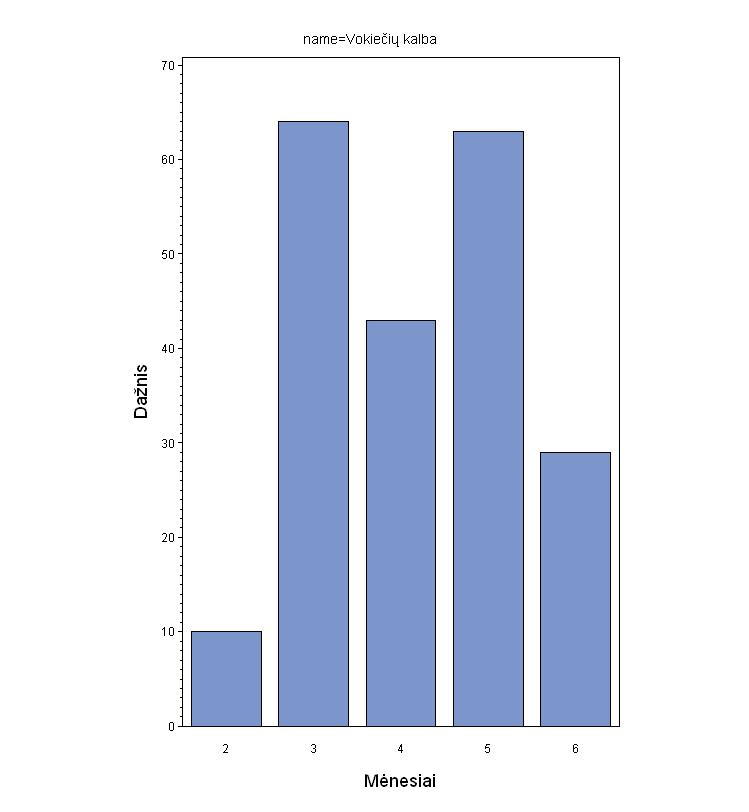
\includegraphics[width=0.3\linewidth]{%
    images/months/Vokieciu_kalba.png}}

  \caption{Darbo pasiskirstymo semestro metu analizė pagal skirtingus
    dalykus.}
  \label{fig:semester_work}
\end{figure}

\begin{listing}[H]
  \begin{minted}{splus}
  libname proj "C:\SAS\projektas\db";

/* Duomenų tvarkymas. */
data proj.visi;
format duration time8. start_date yymmdd10.;
set proj.visi;
duration=(stop_time - start_time);
month = month(start_date);
run;

/* Darbo pasiskirstymas pagal mėnesius. */
axis1 label = (a=90 height = 1.25 'Dirbtų valandų kiekis');
axis2 label = (height = 1.25 'Mėnesiai');

proc gchart data=proj.visi noprint;
vbar month /
  discrete
  sumvar=duration
  type=sum
  raxis=axis1
  maxis=axis2
  ;
by name;
run;
quit;

proc means data=proj.visi noprint;
var duration;
output out=proj.sum_month sum=sum;
by name month;
run;
  \end{minted}
  \caption{SAS programa naudota pasiskirstymų analizei.}
  \label{lst:months}
\end{listing}
